\chapter{Background}
\label{chap:backgnd}
\begin{abstractchap}
This chapter goes into detail about theoretical axes of this dissertation. First, we present language representations and specifically the three different types that interest us: lexical, syntactic and semantic. Secondly, we cover how we can infer relatedness among words based on the neighbors of each word. This intuition is expressed by the distributional hypothesis. Thirdly, we explain how  we can join words together through their common features by means of a graph-like structure. This structure is known as a language network. Fourth, we detail the techniques used in the multimedia literature to combine (or fuse) features coming from different sources and improve the performance of a knowledge-discovering system. In our work, instead of combining different multimedia sources, we combine diverse textual representations. Finally, we explain the (supervised and unsupervised) methods we employ to solve the NLP tasks at hand.
\end{abstractchap}
\minitoc

\section{Distributional Hypothesis}
The work we present in this thesis is prominently based on the distributional hypothesis (DH). This is also the case for the large majority of semantic approaches in NLP today. This context-analysis insight is usually credited primarily to \cite{harris1954}. The hypothesis is simple yet powerful: it can be formulated as "You shall know a word by the company it keeps." \cite{firth57synopsis}. More formally, it states that the similarity of meaning correlates with the similarity of the word's context distribution. It follows that the meaning of a word can be determined by the set of contexts in which it occurs in a corpus. Consequently, for two target words, the larger the number of shared contexts, the semantically closer these words are. 

\begin{figure}
\centering
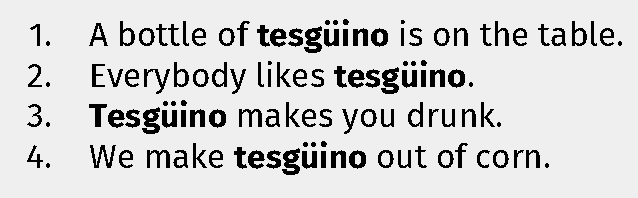
\includegraphics[width=.6\linewidth]{images/Chapitre2/tejuino.pdf}
\caption{Even though \textit{tesg\"{u}ino} is a relatively obscure word, from its context we can understand its an alcoholic drink made from corn.}
\label{fig:tejuino}
\end{figure}


Taking the classic example by \cite{nida1979componential}, shown in the four lines  in Figure \ref{fig:tejuino}, even if we do not know that the word tesg\"{u}ino (or tejuino) refers to a ceremonial corn beer consumed by the native people of the north of Mexico, we can infer, by looking at its context, that we are indeed referring to some sort of corn alcoholic beverage. We can then easily infer that tesg\"{u}ino is similar to other drinks such as tequila or mezcal.

Although we usually find in the literature that the work of Harris is the most important concerning the DH, we should note that the hypothesis rests on two theories  \cite{sahlgren2008distributional,turney2010}: the statistical semantics hypothesis \cite{booth1955machine}, and the  structuralism theory, as described by \cite{de1916course}. The former is important as it place the DH in a within a larger context. Broadly, it affirms that statistical patterns of human word usage can be employed to understand what people mean. The latter,  gives the DH a more robust approach towards the definition of what kind of distributional context should we use to determine similarities, as well as what does it the meaning of the contextual relations between words. In plain words Saussure's version of the structuralist theory indicates that the differences in the contexts of a word determine its role within a language system. 

To this end, Saussure proposed two kinds of context relations: syntagmatic and paradigmatic. Syntagmatic relations concern the context defined by words that co-occur in the text, such as collocations (multi-word expressions that occur frequently in a corpus) and colligations (relations between a lexical item and a grammatical category) \cite{verschueren2015handbook}. On the other hand, paradigmatic relations associate words according to whether they appear or not in the same context. These contexts define classic semantic relations such as synonymy-antonymy or hypernymy-hiponymy. Coupling both the DH with structuralist theory gives birth to the more refined definition of the distributional hypothesis, introduced by \cite{sahlgren2008distributional}: the refined distributional hypothesis. We note that this distinction, syntagmatic versus paradigmatic relations, is also more recently defined in \cite{schutze1993vector}. In their work, syntagmatic relations are called first-order co-occurrences, while paradigmatic relations  are referred to as secord-order co-occurrences.

\begin{figure}
\centering
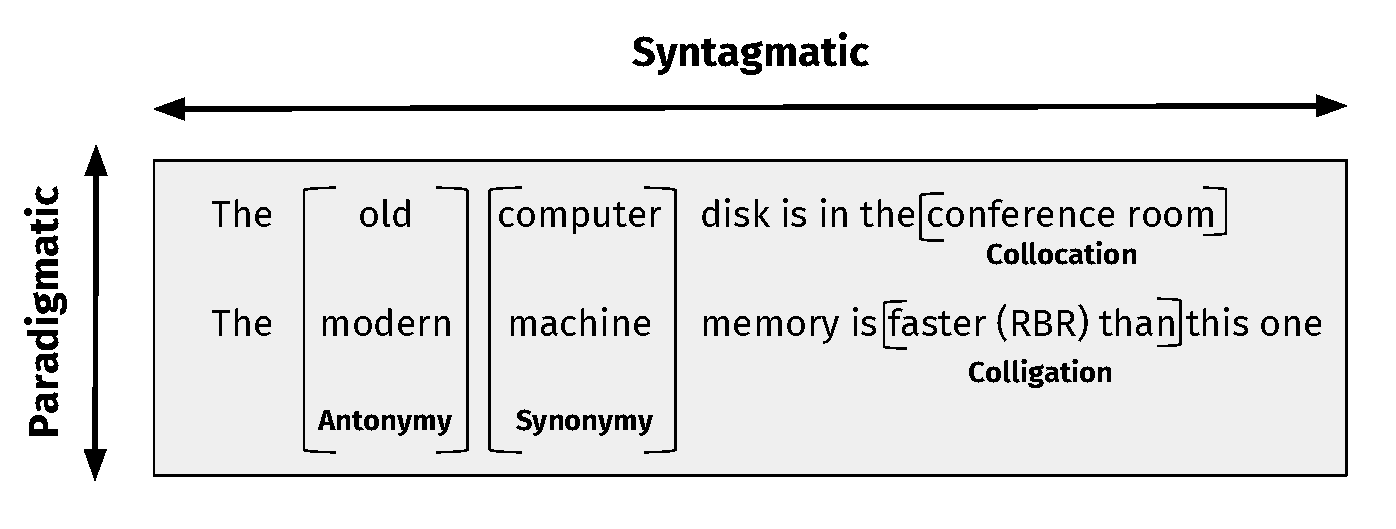
\includegraphics[width=\linewidth]{images/Chapitre2/sintagmatic_paradigmatic.pdf}
\caption{Examples of syntagmatic and paradigmatic contexts and their corresponding semantic relationships. Based on the examples by \cite{sahlgren2008distributional,piero2017}.}
\label{fig:sintagmatic_paradigmatic}
\end{figure}


An example of syntagmatic and paradigmatic relationships can be seen in Figure \ref{fig:sintagmatic_paradigmatic}. Vertically looking at the words,  \textit{old} and \textit{modern}, in the first and second phrase respectively,  share a paradigmatic context which leads to an antonym semantic relation. Something similar happens with words \textit{computer} and \textit{machine}, this time sharing a synonym relation. With respect to the syntagmatic relationships, horizontally looking at the words, we find the collocation \textit{conference room} in the first phrase, as well as the colligation in the second expression between the word \textit{than} usually preceded by a  comparative adverb (RBR), \textit{faster} in this case. 

In spite of Sahlgren's  distributional hypothesis definition, determining the types and meaning of semantic relations, obtained with distributional methods, is still an open challenge on distributional models and methods. Determining the specific type of semantic relation (e.g., synonymy, hyponymy, meronymy) is still an open issue in the community \cite{turney2010,fabre2015,perinet2015}. While distributional models can give us fast access  to semantic relations between words within a corpus, they are most of the times ambiguous relations. It is still our task, as users, to determine the type of semantic relations found, in the case these distinctions are needed by the NLP system  at hand.
% We note that our work does not delves into the study of the semantic relations but we use them to relate 

Distributional methods, based on the DH, have been used for a long time now \cite{JurafskyM09}, although computationally automatized since the 1990s \cite{perinet2015}. Being a mature research field, systems based on these distributional models are varied and cover a large range of NLP tasks being obviously most popular on semantic tasks \cite{baroni2010distributional}. We do note that nowadays, they have somewhat resurfaced (although they really never went away) thanks to the recent re-introduction of word embeddings, or simply word distributional representations. In short, a word embedding, in the context of newer developments, is a vectorial representation  that "embeds" words into a low-dimensional space, usually generated either by means of some sort of matrix reduction \cite{lebret2013deep,levy2014neural} or by using neural networks \cite{Collobert2011,mikolov2013distributed}. These representations are usually obtained from very large bodies of text and they have shown to be quite effective for solving NLP tasks.

\subsection{Implementation}
We move now onto the description of what are the types of contexts commonly used while implementing a distributional model to represent words. In this work we will exclusively focus on paradigmatic contexts. We will cover two types: lexical co-occurrence and syntactical co-occurrence. The first one describes a word's context based on its nearby words.  The second defines a word's context according to the syntactic relations between the word and its neighbors. We will use the example phrases in Figure \ref{} to illustrate the kind of context we will describe below. The target word in this example is \textit{chip}.
\begin{figure}
\centering
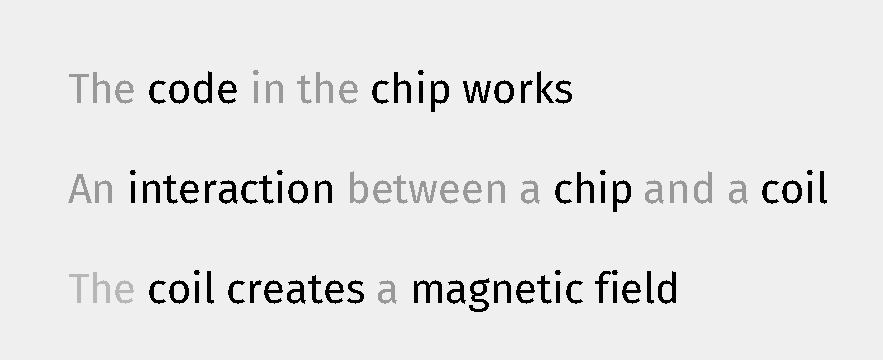
\includegraphics[width=0.7\linewidth]{images/Chapitre2/example_phrases.pdf}
\caption{Example text. Functional words are grayed-out. }
\label{fig:example_phrases}
\end{figure}



\paragraph{Lexical Contexts}
Lexical context, also often called linear contexts  words that co-occur with a target word in a predetermined neighborhood: either in a sentence, a paragraph or larger units of text such as full documents \cite{LevyG14,sahlgren2008distributional}. Nowadays, the lexical context is usually determined by a window of $n$ tokens to each side of the target word. An example of a lexical context is shown in Table \ref{tab:lexical_ex1}. The size of the context depends of course of the application of the system. Indeed, determining the size  is actually a quite empirical decision. Nonetheless, it seems that today the literature \cite{Daume2006,mikolov2013distributed,LevyG14,levy2014neural}  has settled for a two-words to the left and two-words to the right context window, otherwise represented as -2+2. \cite{sahlgren2006word} discusses  the motivations of selecting a window of a particular size. He notes that given the literature evidence,  a shorter context window (specifically a -2+2 window) is preferable for acquiring semantic information. In this sense, \cite{JurafskyM09} sets the generally used context size between 1 and 8 words on each side. In practical terms, the choice of the size  affects the scope of the semantic relatedness: the shorter the context, the more specific is the information about a target word. On the contrary, the larger the window, the broader the information conferred by the context words. 

\begin{table}[]
\centering
\caption{Lexical contexts for the phrases in Figure \ref{fig:example_phrases}. The context is paradigmatic, the window being the complete phrase where the word occur.}
\label{tab:lexical_ex1}
\begin{tabular}{@{}lrrrrrrrrr@{}}
\toprule
       & code & chip & works & interaction & between & coil & creates & magnetic & field \\ \midrule
code        & 0    & 1    & 1     & 0           & 0       & 0    & 0       & 0        & 0     \\
chip        & 0    & 0    & 0     & 1           & 1       & 1    & 0       & 0        & 0     \\
works       & 1    & 1    & 0     & 0           & 0       & 0    & 0       & 0        & 0     \\
interaction & 0    & 1    & 0     & 0           & 1       & 1    & 0       & 0        & 0     \\
between     & 0    & 1    & 1     & 1           & 0       & 1    & 0       & 0        & 0     \\
coil        & 0    & 1    & 0     & 1           & 1       & 0    & 1       & 1        & 1     \\
creates     & 0    & 0    & 0     & 0           & 0       & 0    & 0       & 1        & 1     \\
magnetic    & 0    & 0    & 0     & 0           & 0       & 0    & 1       & 0        & 1     \\
field       & 0    & 0    & 0     & 0           & 0       & 1    & 1       & 1        & 0     \\ \bottomrule
\end{tabular}
\end{table}


Lexical co-occurrences are the most popular way to represent distributional contexts. They are easy to obtain as there is no need for external information except the input corpus itself. We may apply a filter to determine which words we want to include in our context windows. For example, by previously applying a part of speech tagging to the text, we can choose to work only with the nouns or the adjectives. 

 

\begin{figure}
\centering
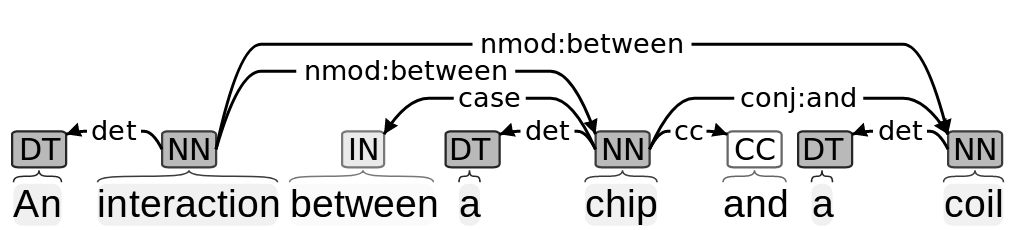
\includegraphics[width=0.9\linewidth]{images/Chapitre2/exo1_dependences.png}
\caption{}
\label{fig:exo1_dependences}
\end{figure}

\begin{figure}
\centering
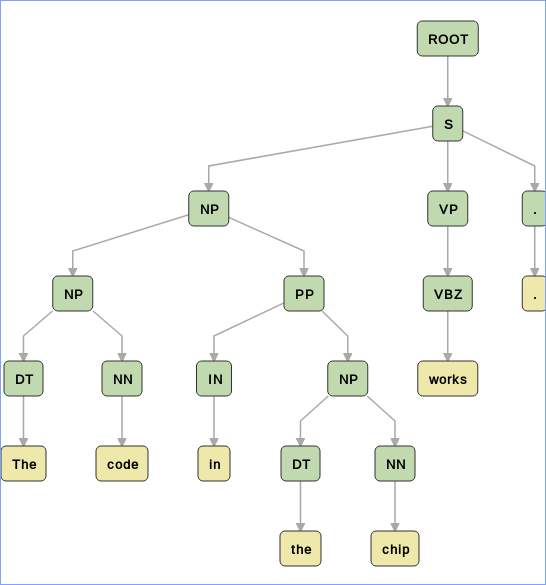
\includegraphics[width=0.7\linewidth]{images/Chapitre2/exo1_constits.png}
\caption{}
\label{fig:exo1_constits}
\end{figure}


%\subsection{Lexical Representations}
%\subsection{Syntactic Representations}
%
 

\paragraph{How do we represent this distributaniolity? }
 context. The most basic form of co-occurrence is determined by neighbor words that appear before or after a word of interest. 
The propositions we present in this thesis are greatly based on the analysis of a word context as a source of valuable information   to discover its nature. 

The distributional hypothesis is popularly exploited in the NLP/Text mining domain by using the vector space model. In this model a word is represented by a vector in which the elements are derived from the occurrences of the word in various contexts, such as windows of words ($n$-words to the right and to the left), syntactical positions or grammatical dependencies,  among other contexts. In our research we chose not to use vectors directly but instead use graphs (and hypergraphs) as an intuitive way to model the context of words in a corpus. Graphs have the capability to naturally encode the meaning and structure of a text by connecting language units (words in our case) through various relationships. Indeed, recent years have seen a rise in natural language methods based on graph-theoretical frameworks \cite{Mihalcea2011}. Specifically, in this work we represent words as vertices and the edges that link these nodes (words) correspond to various linguistic context properties shared among them. 


%
%
%
%
%
%\section{Vector Space Model and Graph-based representations}
%\subsection{Vector Space Model}
%\subsection{Graph-based Models}
%
%
%
%\section{Supervised and Unsupervised Methods}
%\subsection{Supervised Methods}
%\subsubsection{Logistic Regression}
%\subsubsection{Structured Perceptron}
%\subsection{Unsupervised Methods}
%\subsubsection{Spectral Clustering}
%
%\section{Word Sense Induction and Disambiguation}
%\section{Named Entity Recognition}

%++++++++++++++++++++++++++++++++++++++++++++++++++++++++++++++++++++++++++++++++++++++++++++++++++



